\section{Introduction}

% General paragraph on AD
Alzheimer's Disease (AD) is a neurodegenerative disease that causes progressive cognitive impairment, leading to death \cite{Lane2018}. AD currently has no cure and puts a strong strain in healthcare systems, due to the care needed by patients at later stages of the disease \cite{AlzheimersAssociation}. AD is a multifactorial disease that affects different systems and processes of the brain \cite{Jack2010}. Those processes are captured using different biomarkers coming from various imaging modalities, such as magnetic resonance imaging (MRI) to capture atrophy or positron emission tomography (PET) for glucose uptake or blood flow. For a disease as complex as AD, it is necessary to study not only how those different biomarkers interact between each other, but also their progression over time. For this reason, the use of longitudinal data, captured over several time points, is extremely valuable to researchers. However, it is often difficult to use this kind of medical data, as it can present missing data across modalities (e.g. unwillingness of  patients to receive invasive testing or unfeasibleness due to health concerns) and over time (e.g. due to medical follow-ups that were missed). \\

% Introduction to disease progression methods (probably would be removed in a journal paper).
Modelling longitudinal, multivariate data is a difficult task \cite{Verbeke2014}. For neurodegenerative diseases, progression modelling methods can be used to leverage medical data to identify and predict the trajectories of biomarkers, which could lead to better characterization and understanding of the evolution of the disease. Such techniques have been used for many degenerative diseases, including AD \cite{Oxtoby2017,Marti-Juan2020}. Examples of those techniques include event-based models \cite{Young2014,Young2015a,Fonteijn2012}, which discover, for a set of biomarkers, the order in which they will degenerate; Gaussian processes \cite{Lorenzi2015b,Hyun2016,Lorenzi2019}, which allow characterizing the uncertainty of the progression; and other methodologies \cite{Marinescu2019, Young2017}. Cao et al.\ \cite{Cao2019} proposed a method using canonical correlation analysis to compare two different time series, applied to functional MRI analysis. More recently, Antelmi et al.\ \cite{Antelmi2019} proposed a generative method based on a multi-channel variational autoencoder (VAE) using multiple modalities of cross-sectional data. Their method inferred a lower dimensional latent space generated jointly from all the modalities, and it modelled the dependence across modalities, being able to generate those that were missing in specific patients. These methods, however, are usually limited in the number of modalities they can combine or in the amount of longitudinal data they use (cross-sectional data, or only short-term data). Moreover, it is not clear how to combine longitudinal modalities with non-temporal ones, such as demographic or genetic data, which can influence the trajectory of the disease. \\

Longitudinal data can also be processed as sequences of data. Recurrent neural networks (RNN) \cite{Hochreiter1997} have become a powerful tool for sequence learning in the past few years. Although they have been mainly used for natural language processing \cite{Goldberg2017}, they have also been applied in other fields, such as image generation \cite{Gregor2015a} and AD progression \cite{Wang2018,Ghazi2019}. Variational RNN \cite{Chung2015,Fabius2015} adds a variational component to the RNN arquitecture, allowing it to capture more complex temporal variation by setting dependencies across time between the random latent variables. \\ 


In this chapter, we propose a multi-channel recurrent variational autoencoder  (MC-RVAE) for disease progression modelling. Similarly to \cite{Antelmi2019}, we jointly model the dependencies across the channels of the network, but we build on the model by adding a variational recurrent block to capture the temporal dependencies alongside every channel. The model is able to use longitudinal data with variable number of time points and missing modalities. We show that the model captures the progression of the disease and the relationships between the modalities, being able to reconstruct missing modalities and predict future time points. Results shown in this chapter are preliminary at the time of writing this thesis, and more research is being conducted to improve and extend them. \\

%% Needs to be updated when the whole chapter is detailed
The chapter is organized as follows: In Section \ref{rnn:background}, we give some background on recurrentneural networks and variational autoencoders. In Section \ref{rnn:methods} we detail the proposed method, derive the variational lower bound used to optimize the model, and detail the experiments conducted, as well as the data used. Section \ref{rnn:results} contains the detailed results of our experiments. In Section \ref{rnn:discussion} we discuss the current results and show the most important contributions. Finally, in Section \ref{rnn:conclusions} we summarize the chapter, address the limitations of our model, and propose future lines of research.

\section{Background}
\label{rnn:background}

\subsection{Recurrent neural networks}

RRNs are a family of neural networks that are able to model sequences by recursively processing the input data, using previous outputs as inputs. They can achieve that by maintaining a hidden state $h$, a variable that can store information of the sequence. This makes this type of network ideal for temporal sequences. A basic RNN architecture can be described as:

\begin{equation}
    h_t = \mathit{\sigma}(W_h h_{t-1} + W_x x_{t} + b_h),
    %& y_t = \mathit{\sigma_y}(W_y h_t + b_y),
\end{equation}

where $x_t$ is the vector of data at time $t$ and $h_{t-1}$ is the hidden state of the recurrent network at time $t-1$. $\sigma$ is a non-linearity, whereas $W_h$, $W_x$ and $b_h$, $b_x$ are the weights and biases of the network, respectively. RNN are recurrent networks in the sense that each subsequent state $h_t$ depends on all previous ones. Figure \ref{fig:rnnvae:rnn} shows this recurrence and how it unrolls for a single RNN for an input sequence $x = (x_0,x_1, ..., x_t)$. \\

\begin{figure}[!htbp]
  \centering
  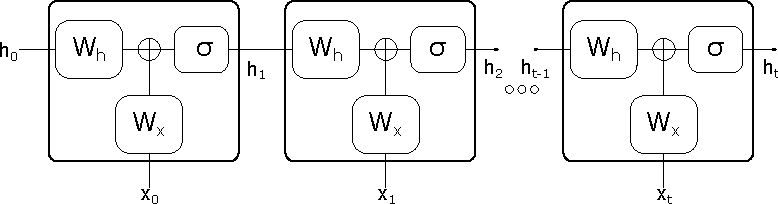
\includegraphics[width=0.9\textwidth]{figures/rnnvae/rnn-fig.pdf}
  \caption[Unroll of the recurrency for a basic RNN.]{Unroll of the recurrency for a simple RNN and input sequence $x = (x_0,x_1, ..., x_t)$. $W_h$ and $W_x$ are weight matrices. Biases not shown in the figure.}\label{fig:rnnvae:rnn}
\end{figure}

This is the basic formulation of a RNN, and although it works well for short-range sequences, it can fail for longer sequences due to gradient vanishing \cite{Hochreiter1998}, caused by the large number of operations needed to compute the gradient during training. More complex formulations have been proposed in the literature to address those issues, such as LSTM \cite{Hochreiter1997} or GRU \cite{Chung2014}. For a more in-depth look at RNNs, including training, formulation and derivation, we refer the reader to \cite{Sherstinsky2020}.  \\

\subsection{Variational autoencoders}

Variational autoencoders (VAE) are probabilistic models that encode the observed input $x$ into a vector of latent random variables $z$, creating a low-dimensional variational latent space that captures the main variations present in the input space and allows for sampling and inference. The joint probability of a standard VAE is:

\begin{equation}
    p(x,z) = p(x|z)p(z),
\end{equation}

where $p(x|z)$ is the likelihood of the input data conditioned on $z$ and $p(z)$ is the prior distribution of the latent variable. We want to infer the posterior $p(z|x)$, which will give us the best $z$ distribution for our data:

\begin{equation} \label{eq:rnnvae:intract}
\begin{aligned}
p(z|x) = \frac{p(x,z)}{p(x)}, \\
\text{with } p(x) = \int p(x,z) dz.
\end{aligned}
\end{equation}

However, this posterior cannot be computed directly for most problems, as $\int p(x)$ is intractable for most complex distributions. To solve this, we perform variational inference by approximating the real posterior by another distribution. We call this the approximate posterior $q(z|x)$. We define the objective function as:

\begin{equation}
\ln p(x) = \int \ln p(x,z) \,dz,
\end{equation}

We can use a lower bound on this expression to define an optimization objective that is tractable: 

\begin{equation}
    \ln p(x) \geq \mathbb{E}_{q(z|x)} \ln(p(x|z)) - \mathcal{D}_{KL}(\infdiv{q(z|x)}{p(z)}),
\end{equation}

where $D_{KL}$ is the Kullback-Leibler (KL) divergence. The full derivation of this lower bound can be found on \cite{Kingma2014}. The first term of this lower bound is the (negative) reconstruction error, which favors maximizing the expected log likelihood of the data, whereas the second term is the regularization term, which represents the divergence between the encoder and the prior of the latent space (usually a normal distribution). This term forces the latent distribution not to directly encode an identity between input and output. \\

Variational auto-encoders can be parametrized by defining $p(x|z)$ and $q(z|x)$ as neural networks (usually called the decoder and encoder, respectively), and we can train their associated parameters using gradient descent by optimizing the lower bound. However, directly sampling from the encoder $z\sim q(z|x)$ leads to high variance estimates of the gradient and makes training very difficult. To solve this, Kingma et al.\ \cite{Kingma2015} proposed to reparametrize the estimation by introducing a random variable from a simple distribution $\varepsilon \sim N(0,I)$ and mapping it to $z$. For example, if $q(z|x)$ is parametrized as a normal distribution $\mathcal{N}(\mu, \Sigma)$:

\begin{equation}
\begin{split}
    \varepsilon \sim \mathcal{N}(0,I) \\
    z = \mu + \Sigma \cdot \varepsilon
\end{split}
\end{equation}

This approach leads to a lower variance estimator and allows for a smooth training.

\section{Methods}
\label{rnn:methods}

\subsection{MC-RVAE: multi-channel recurrent variational autoencoder}

% T can be variable across channels. Should I put this?
Let $x = (x^0,...,x^c,...,x^{C-1})$ be a set of data sequences across $C$ different channels. Each of these sequences are defined over $T$ time points  $x^c = (x^c_{0},...,x^c_{t},...,x^c_{T-1})$. For readability, in our notation, we assume that all the channels have the same number of time points. We base our model on two assumptions: the existence of temporal dependencies across time steps for each different channel $x^c$, and cross-channel dependencies, both contributing to the underlying joint trajectory of the disease. To capture the temporal dependencies, we use a variational RNN, similar to the one described in \cite{Chung2015}, where we generate latent variables $z_t$ at each timestep $t$, which are conditioned on the hidden states of the RNN at the previous temporal step $h_{t-1}$. For the inter-channel dependencies we assume, similarly to \cite{Antelmi2019}, that each channel $x^c$ share the same latent space $z$, and that each channel is conditionally independent from the others. \\

We first describe the encoder and the decoder of our model for a specific channel $c$ and time point $t$:

\begin{equation} 
\begin{aligned} \label{rnn:eq:generative}
\displaystyle
& \mathit{p}(x^c_t | z_{\leq t}, x^c_{< t}) = \mathcal{N}(\mu_{x^c_t},\Sigma_{x^c_t}), \text{ where } [\mu_{x^c_t},\Sigma_{x^c_t}] = \varphi_{dec}(\varphi_{z}(z_t), h_{t-1}) \\
& \mathit{q}(z_t | x^c_{\leq t}, z_{< t}) = \mathcal{N}(\mu_{z,t},\Sigma_{z,t}), \text{ where } [ \mu_{z,t},\Sigma_{z,t}] = \varphi_{enc}(\varphi_{x^c}(x^c_{t}), h_{t-1}) \\
\end{aligned}
\end{equation}

% Explanation of all the small things
The first line of Equation \ref{rnn:eq:generative} corresponds to the approximate posterior or decoder, defined by a normal distribution parametrized by $\varphi_{dec}$, which can be any differentiable function (for example, a neural network). The second line corresponds to the encoder, defined similarly to the decoder. They both include as a parameter $h_{t-1}$, which is the hidden state of the previous recurrent step. $z$ and $x$ are also transformed by $\varphi_{z}$ and $\varphi_{x^c}$, differentiable functions, with $\varphi_{x^c}$ being specific to each channel. These transformations are key for the network to learn complex sequences \cite{Chung2015}.\\

The recurrent step is defined by:

\begin{equation} 
\begin{aligned} \label{rnn:eq:recurrent}
h_{t} = \mathit{f}_{\theta}(\varphi_{x^c}(x^c_{t}), \varphi_{z}(z_t), h_{t-1}), \\
\end{aligned}
\end{equation}

where $\mathit{f}_{\theta}$ can be parametrized by any recurrent architecture. We can then define the prior of $z_t$ as:

\begin{equation}
\begin{gathered} \label{rnn:eq:prior} 
z_t \sim \mathcal{N}(\mu_{0,t},\Sigma_{0,t}), \text{ where } [\mu_{0,t},\Sigma_{0,t}] = \varphi_{prior} (h_{t-1}), \\
\end{gathered}
\end{equation}

where $h_{t-1}$ is the hidden state of the channel at the previous time point. Note that both the encoder and the decoder depend on $h_{t-1}$, which make each output at a step $t$ dependant on $t-1$, with $h$ modelling this relationship. \\

Accounting for the dependencies described by the recurrent step in Equation \ref{rnn:eq:recurrent}, for any time point $T>0$, and for a specific channel, the encoder and decoder can be factorized as:

\begin{equation} \label{eq:decfact}
\mathit{q}(z_{\leq T} | x^c_{\leq T}) = \prod^T_{t=1} \mathit{q}(z_t | x^c_{\leq t}, z_{<t})
\end{equation}

\begin{equation} \label{eq:encfact}
    \mathit{p}(x^c_{\leq T}, z_{\leq T}) = \prod^T_{t=1} \mathit{p}(x_t | z_{\leq t}, x^c_{<t})\mathit{p}(z_t | x^c_{<t}, z_{<t}).
\end{equation}

These expressions will be used for the derivation of the lower bound of the model. Figure \ref{fig:rnn} shows a visual representation of the main recurrent building block of the network.

\begin{figure}[!htbp]
  \centering
    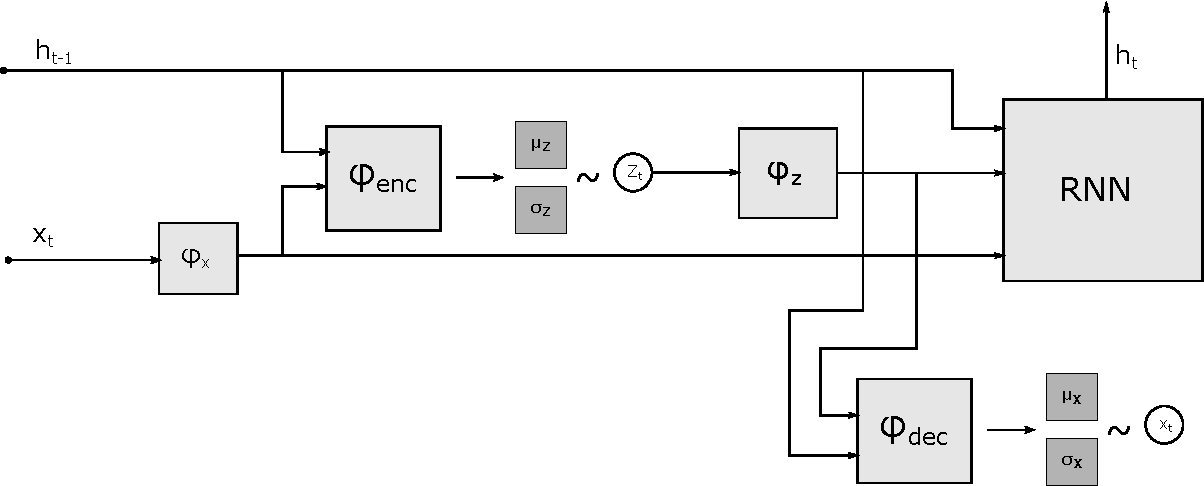
\includegraphics[width=0.9\textwidth]{figures/rnnvae/Fig1.pdf}
  \caption[Building block of the network, for a single channel.]{Building block of the network, for a single channel (channel label not included for clarity). $x_t$ is the input at time-step $t$, and $h_t$ is a hidden state of the RNN. }\label{fig:rnn}
\end{figure}

\subsubsection{Derivation of the lower bound}
The optimization objective of MC-RVAE is the evidence lower bound (ELBO) \cite{Kingma2014} of the log likelihood of the data. We can define it as:

\begin{equation}
    \ln \mathit{p}(x_{\leq T}) = \ln \int \mathit{p}(x_{\leq T}, z_{\leq T}) \,dz_{\leq T},
\end{equation}

over all time points. Multiplying it by $\mathit{q}(z_{\leq T}|x^c_{\leq T})$, over all channels:

\begin{equation}
= \mathbb{E}_c \ln \int \mathit{p}(x_{\leq T}, z_{\leq T}) \frac{\mathit{q}(z_{\leq T}|x^c_{\leq T})}{\mathit{q}(z_{\leq T}|x^c_{\leq T})} \,dz_{\leq T},
\end{equation}

and, by Jensen's inequality, we obtain a lower bound:

\begin{equation} 
\begin{aligned}
\displaystyle
    \geq \mathbb{E}_c \int \mathit{q}(z_{\leq T}|x^c_{\leq T}) \ln \left( \frac{\mathit{p}(x_{\leq T},z_{\leq T})}{\mathit{q}(z_{\leq T}|x^c_{\leq T})} \right) \,dz_{\leq T}.
\end{aligned} \label{rnn:eq_loglike}
\end{equation}

We can decompose this expression by factoring the terms inside the logarithm, using Equations \ref{eq:decfact} and \ref{eq:encfact}:

\begin{equation} 
\begin{aligned}
\displaystyle
= \mathbb{E}_c \int \mathit{q}(z_{\leq T}|x^c_{\leq T}) \ln \left( \prod^T_{t=1} \frac{\mathit{p}(z_t |x_{< t}, z_{< t})\mathit{p}(x_t |z_{\leq t}, x_{< t})}{\mathit{q}(z_t |x^c_{\leq t}, z_{< t})} \right) \,dz_{\leq T}
\end{aligned}
\end{equation}

\begin{equation} 
\begin{aligned}
\displaystyle
= \mathbb{E}_c \int \mathit{q}(z_{\leq T}|x^c_{\leq T}) \sum^T_{t=1} \ln \left( \frac{\mathit{p}(z_t |x_{< t}, z_{< t})\mathit{p}(x_t |z_{\leq t}, x_{< t})}{\mathit{q}(z_t |x^c_{\leq t}, z_{< t})} \right) \,dz_{\leq T}
\end{aligned}
\end{equation}

\begin{equation} 
\begin{aligned}
\displaystyle
= \mathbb{E}_c  \sum^T_{t=1} \Big[ & \int \mathit{q}(z_{\leq t}|x^c_{\leq t}) \ln \left( \frac{\mathit{p}(z_t |x_{< t}, z_{< t})\mathit{p}(x_t |z_{\leq t}, x_{< t})}{\mathit{q}(z_t |x^c_{\leq t}, z_{< t})} \right)\, dz_{\leq t} \\
& \int \prod^T_{t'=t+1} \mathit{q}(z_{t'}|x^c_{\leq t'}, z_{<t'}) \, dz_{>t} \Big] \\
\end{aligned}
\end{equation}

\begin{equation} 
\begin{aligned}
\displaystyle
= \mathbb{E}_c \sum^T_{t=1} \int \mathit{q}(z_{\leq t}|x^c_{\leq t}) \ln \left( \frac{\mathit{p}(z_t |x_{< t}, z_{< t})\mathit{p}(x_t |z_{\leq t}, x_{< t})}{\mathit{q}(z_t |x^c_{\leq t}, z_{< t})} \right)\, dz_{\leq t}.
\end{aligned}
\end{equation}


We decompose the expression inside the logarithm to obtain:

\begin{equation} 
\begin{aligned}
\displaystyle
= \mathbb{E}_c \sum^T_{t=1} \Big[ & \int \mathit{q}(z_{\leq t}|x^c_{\leq t}) \ln \mathit{p}(x_t |z_{\leq t}, x^c_{< t})  \,dz_{\leq t} \\
&+ \int \mathit{q}(z_{\leq t}|x^c_{\leq t}) \ln \frac{\mathit{p}(z_t |x_{< t}, z_{< t})}{\mathit{q}(z_t |x^c_{\leq t}, z_{< t})} \,dz_{\leq t} \Big].
\end{aligned}
\end{equation}

As we can factorize $\mathit{q}(z_{\leq t}|x^c_{\leq t}) = \mathit{q}(z_t |x^c_{\leq t}, z_{< t})\mathit{q}(z_{< t}|x^c_{< t})$, the second term is the expectation of the negative KL divergence between the approximate posterior and the true one, over $\mathit{q}(z_{< t}|x^c_{< t})$:

\begin{equation} 
\begin{aligned}
\displaystyle
= \mathbb{E}_c \sum^T_{t=1} \Big[  & \int \mathit{q}(z_{\leq t}|x^c_{\leq t}) \mathit{p}(x_t |z_{\leq t}, x_{< t}) dz_{\leq t} \\
&- \int \mathit{q}(z_{< t}|x^c_{< t}) \mathcal{D}_{KL}(\mathit{q}(z_t |x^c_{\leq t}, z_{< t}) || \mathit{p}(z_t |x_{< t}, z_{< t})) \,dz_{< t} \Big],
\end{aligned}
\end{equation}

which finally leads to:

\begin{equation} 
\begin{aligned}
\displaystyle
= \mathbb{E}_c \,\mathbb{E}_{\mathit{q}(z_{\leq T}|x^c_{\leq T})}  \Big[ & \sum^T_{t=1} \ln \mathit{p}(x_t |z_{\leq t}, x_{< t}) \\
&- \mathcal{D}_{KL}(\mathit{q}(z_t |x^c_{\leq t}, z_{< t}) || \mathit{p}(z_t |x_{< t}, z_{< t})) \Big].
\end{aligned}
\end{equation}

As the channels are conditionally independent from the others, we can factorize the log likelihood over each individual channel as:

\begin{equation} 
\begin{aligned} \label{rnn:eq:finalopt}
\displaystyle
= \mathbb{E}_c \,\mathbb{E}_{\mathit{q}(z_{\leq T}|x^c_{\leq T})} \Big[ \sum^T_{t=1} & \Big[ \sum^C_{i=1} \ln \mathit{p}(x^i_t |z_{\leq T}, x^i_{< t}) \Big] \\
&- \mathcal{D}_{KL}( \mathit{q}(z_t |x^c_{\leq t}, z_{< t}) || \mathit{p}(z_t |x_{< t}, z_{< t})) \Big].
\end{aligned}
\end{equation}

By maximizing this lower bound with respect to the model parameters, we are also minimizing the log likelihood of the model. The first term of Equation \ref{rnn:eq:finalopt} forces a joint decoding of the channels at each time point, allowing us to predict missing channels. The second term, which acts as a regularization, forces the encoders of each channel to be close to a common prior generated from the previous time point, enforcing a temporal structure.

\subsubsection{Channel reconstruction}

Thanks to the first term of the lower bound in Equation \ref{rnn:eq:finalopt}, we are able to reconstruct the data for a missing channel using existing ones. For a missing channel $c_{m}$, and for each time point $t$, we can decode the associated latent space $z$ of each existing channel and reconstruct the missing channel using the following expression:

\begin{equation}
    x^{c_m}_t = \mathbb{E}_{c} [ \mathbb{E}_{q(z|x^c_t)} \sum p(x^{c_m}_t|z) ].
\end{equation}

\subsubsection{Variational dropout} 

Variational dropout was proposed by Kingma et al.\ \cite{Kingma2015} to regularize variational autoencoders and sparsify their latent space. It works by specifying a reparametrization of the posterior and learning the dropout rates of each latent dimension via a trainable parameter. This reparametrization is defined as:

\begin{equation}
    \mathit{q}(z_t | x^c_{\leq t}, z_{< t}) \sim \mathcal{N}(\mu_{z,t},\alpha\mu_{z,t}^2),
\end{equation}

with $\alpha$ being a learned parameter shared across channels and time points. With this reparametrization, we can use an approximation of $\mathcal{D}_{KL}$, defined in \cite{Kingma2015}, that only depends on $\alpha$. This approximation, however, requires the prior to be improper log-scale uniform. As in our model we have a learned prior for $t>0$ (Equation \ref{rnn:eq:prior}), this assumption can only hold when $t=0$. We experimented with applying this reparametrization and only using the approximation of $\mathcal{D}_{KL}$ for $t=0$. We conducted a number of synthetic and real data experiments to assess the effect of this approach.

\subsubsection{Missing data and variable number of time points}

The described method works when $T$ is the same across channels, and when there are no missing data points. However, with real data, that is not always the case. To account for missing data, for each time point $t$, we limit our optimization over samples that have that time point, doing the same for missing channels. However, this could lead to a bias towards samples with more time points. For this reason, we add a mean term for each subject to both terms of the loss, to make every subject weight equally regardless of their number of time points. \\

In the case where a channel only has a time point (e.g. demographic data, or genetic information, which is not longitudinal), the channel is only included on the optimization when $t=0$, and is considered as a channel with only one time point for all the related calculations.

\subsection{Data}

Experiments on the method were performed on both synthetic and real data. In this section, we describe their characteristics.

\subsubsection{Synthetic data}

We implemented a generation method of longitudinal data from a set of latent variables of fixed dimensionality:

\begin{equation} 
\begin{gathered} \label{rnn:eq:synthdata}
   z \sim \mathcal{N}(0, I_{l}) \\
   \varepsilon \sim \mathcal{N}(0, I) \\
   x^c_t = W^{c}z + f_{long}(t) + \varepsilon
\end{gathered}
\end{equation}

$I_{l}$ is the identity matrix with size $l \times l$, where $l$ is the latent space size. $W^c \in \mathbb{R}^{g \times l}$, with $g$ being the number of features of the output channel, is a random orthonormal matrix that linearly relates each channel $c$ to the latent space.  $f_{long}$ represents the temporal component of the data, depending on time point $t$, and $\varepsilon$ is a random noise variable. We use simple sigmoid, cosinus and sinus functions. Each channel will have a different longitudinal component, depending on a common underlying latent space. We test the performance of variational dropout for different values of $l$. We also evaluate if the network is able to reconstruct the original channel.   \\

\subsubsection{ADNI data}

Data used in this chapter were obtained from the Alzheimer’s Disease Neuroimaging Initiative (ADNI) database \cite{Mueller2005}. The ADNI was launched in 2003 as a public-private partnership led by PI Michael W. Weiner, MD. The primary goal of ADNI has been to test whether serial biological imaging biomarkers, and clinical and neuropsychological assessment can be combined to measure the progression of MCI and early AD. \\

We focused on five different data modalities. Full relation of the features used can be found in supplementary file S1: \\

\begin{itemize}
    \item Brain subcortical volumes: We select MRI T1 weighted images, preprocessed using gradient warping, scaling, B1 correction, and N3 homogeneity correction. Images were then automatically processed with the longitudinal pipeline \cite{Reuter2012} in FreeSurfer. Specifically, an unbiased within-subject template space and image is created using robust, inverse consistent registration \cite{Reuter2010}. Several processing steps, such as skull stripping, Talairach transform, atlas registration as well as spherical surface maps and parcellations are then initialized with common information from the within-subject template, significantly increasing reliability and statistical power. We use the parcelled subcortical volumes, obtaining 40 features.
    \item Cortical thickness: We use the same imaging pipeline described above. We use the parcelled cortical thickness, obtaining 68 features.
    \item Cognitive assessment scores: A set of six different neuropsychological assessment tests that capture the level of cognitive decline of patients in specific tasks and domains. 
    \item Demographic information: three features of demographic information: age at baseline, sex, and years of education of the patient. This is a cross-sectional, baseline modality.
    \item APOE (Apolipoprotein) $\varepsilon4$ allele load: a single feature indicating the number of copies of this allele, which is a risk factor of AD \cite{Saunders1993}. This is a cross-sectional, baseline modality.
\end{itemize}

We selected subjects that had no missing data at their baseline acquisition for any of the channels, and all subsequent follow-ups that had at least one of the existing longitudinal modalities, and had no missing features intra-modality. With this criteria, we selected 897 subjects, with a total of 7224 acquisitions. Table \ref{rnn:demographic} shows the demographic information of the selected cohort. Regarding the distribution of the data across modalities, Figure \ref{fig:rnn:missingdata} shows the information about missing, mean and maximum number of acquisitions across modalities.

\begin{table}[!htbp]
\centering
\resizebox{0.8\textwidth}{!}{%
\begin{tabular}{@{}ccccc@{}}
\toprule
          & CN & MCI & AD & Total \\ \midrule
No. scans  & 229          & 324    & 180 & 897   \\
Age       & $74.62\pm5.26$ & $73.70\pm7.33$ & $73.66\pm7.84$  &  $73.57\pm6.92$     \\
Education & $16.23\pm2.72$ & $15.67\pm2.98$ & $14.95\pm2.93$  &  $15.77\pm2.88$     \\
MMSE      & $29.06\pm1.09$ & $27.13\pm1.80$ & $23.19\pm1.97$  & $27.09\pm2.65$      \\
Female    &  $51.53 \%$   & $40.12 \%$      &  $50.55\%$      &  $46.7\%$    \\
APOE $\varepsilon$4     & $27.51\%$    & $56.17\%$        & $51.1\%$        & $47.8\%$     \\ \bottomrule
\end{tabular}}
\caption[Demographic characteristics of the cohort used, at baseline.]{Demographic characteristics of the cohort at baseline. Age and education presented as average and standard deviation, in years. APOE $\varepsilon$4: Apolipoprotein $\varepsilon$4, percentage with 1 or 2 alleles. CN: Cognitively normal. MCI: Mild cognitive impairment. AD: Alzheimer’s disease. MMSE: Mini-mental state examination. }\label{rnn:demographic}
\end{table}

\begin{figure}[!htbp]
  \centering
  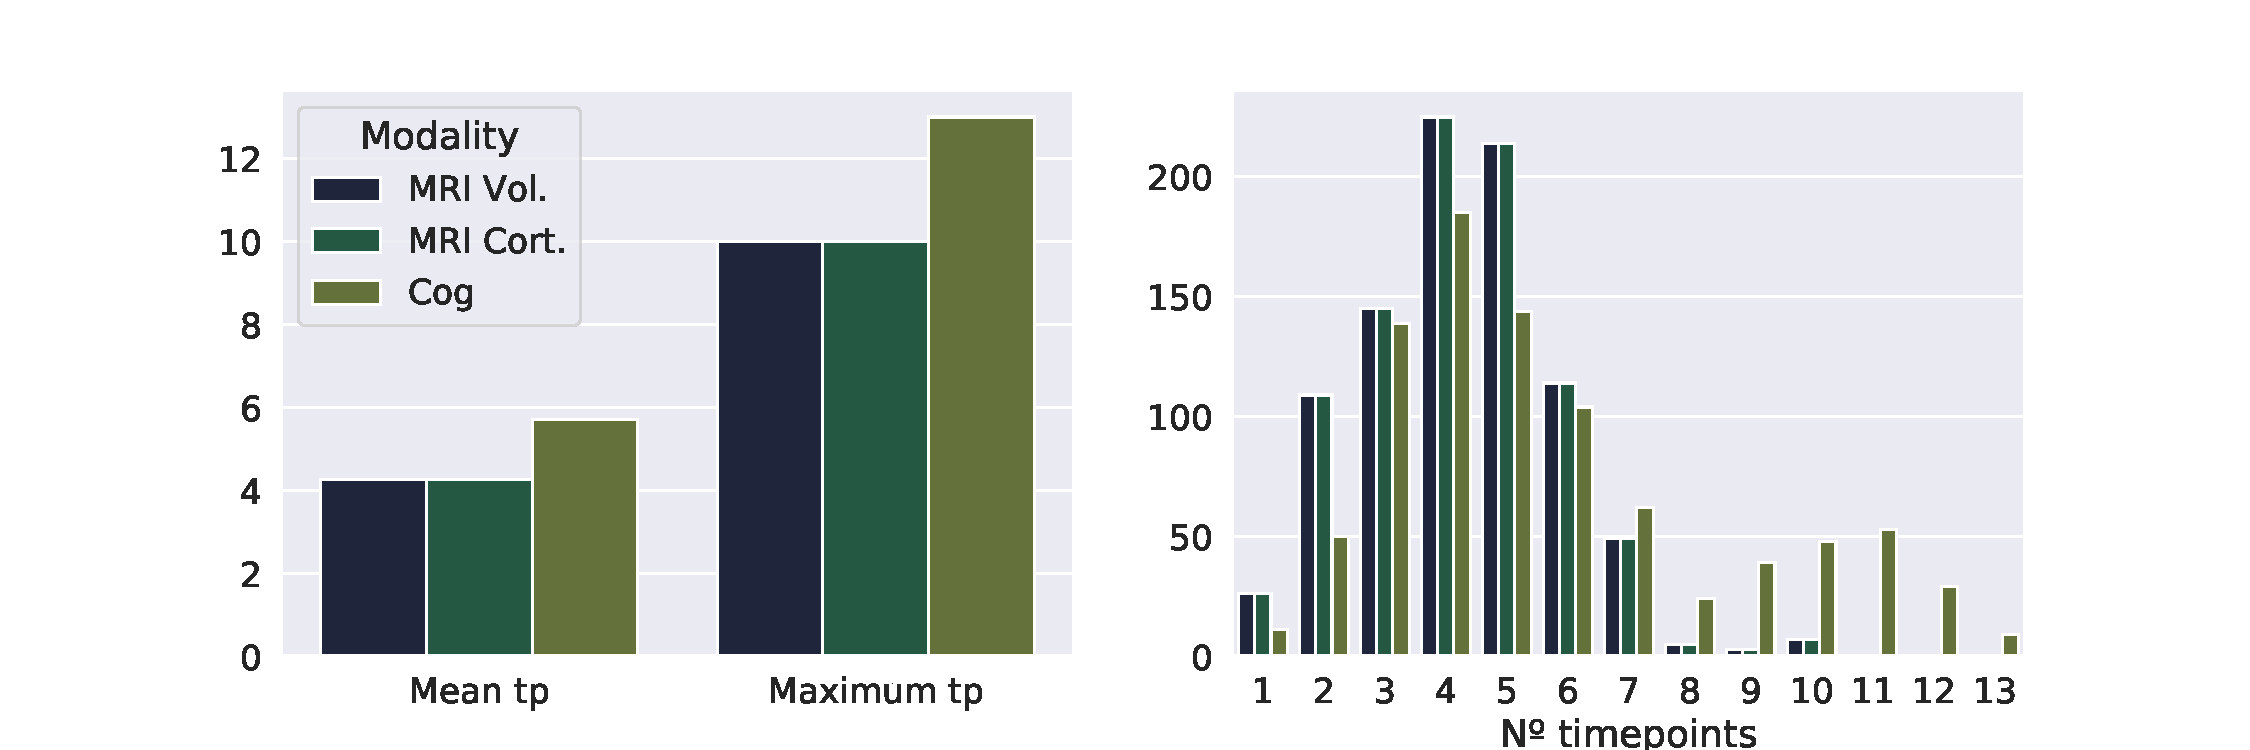
\includegraphics[width=1.0\textwidth]{figures/rnnvae/rnn_long.pdf}
  \caption[Time point distribution of ADNI data.]{Left: mean and maximum amount of time points for the three longitudinal channels. Right: distribution of sequence length across subjects, for each longitudinal channel.}\label{fig:rnn:missingdata}
\end{figure}

Other relevant modalities were considered, such as PET derived biomarkers or cerebrospinal fluid biomarkers, but were ultimately not included due to their low amount of subjects with acquisitions available in the cohort and the low number of follow-ups. \\ 

\subsection{Experiments}

Our experiments with synthetic data are aimed at both showing that the model is able to reconstruct longitudinal signals from missing channels, and to test whether cross-sectional variational dropout would hold for our longitudinal implementation. The parameters used in this model are described in Table \ref{rnn:tablehyper} (first column). We tested for three different real latent dimensions ($l = {2,4,6}$) and observed if the network was able to select a similar number of latent spaces after applying variational dropout. \\

For the ADNI cohort, we first separate our data between training and test set, with 90/10 separation, while maintaining the proportion of diagnosis across sets. The test set is then held out, and we perform an hyperparameter search on the train set using 10-fold cross validation over a set of hyperparameters, shown in Table \ref{rnn:tablehyper} (second column). \\

%%% ACTUALITZAR AL FINAL
\begin{table}[!htbp]
\centering
\resizebox{0.8\textwidth}{!}{%
\begin{tabular}{@{}ccc@{}}
\toprule
Hyperparam & Synthetic model & ADNI model \\ \midrule
Layer size    &   20    & 100, 200, 300  \\
No. latent dim.    &  15   & 10, 20, 30 \\
No. layers    &  1   & 0, 1  \\
RNN hidden size &  30   & 100, 200, 300  \\ \bottomrule
\end{tabular}}
\caption[Hyperparameters of the model.]{Table of hyperparameters. Left column: parameters used with the synthetic model. Right column: parameters used for ADNI model optimization. Layer size: size of all layers in the network (encoder, decoder and $\phi$). RNN hidden: size of the hidden layer in the RNN.}\label{rnn:tablehyper}
\end{table}

The model was trained using gradient descent with Adam \cite{Kingma2015a}, at a learning rate of $1\text{e-}3$ until convergence of the model (roughly 1200 epochs). Code and training settings of the model can be found in the repository of the chapter\footnote{\url{https://github.com/GerardMJuan/RNN-VAE}}. \\

We evaluate our results on the held-out test set on two different tasks: 

\begin{itemize}
    \item \textbf{Time point prediction:} we remove the last time point data from each subject in the test set, and we predict it using the rest of the data. 
    \item \textbf{Channel reconstruction:} we reconstruct each different channel from the rest of the channels, using the joint decoder $p_c(x|z)$. We evaluate the results using different combinations of channels.
\end{itemize}

For the first task, we consider linear regression for each sample and channel as baseline. For the second task, we compare our method to a baseline method based on k-nearest neighbor: for each sample in the test set, we perform a k-means search for each individual channel to find the most similar sample in our training set. For each of those samples, we select the channel we are reconstructing, and we average them to obtain the reconstructed channel for the original sample. We evaluate both tasks using mean absolute error (MAE). \\

We also test the generative capabilities of the model by reconstructing cortical and subcortical data of two synthetic patients: one with a stable, healthy cognitive trajectory, and another one that is rapidly declining. We generate four time points for each of the subjects and visualize the longitudinal neurodegeneration trajectories and their plausibility. Information about the exact data used for those synthetic patients can be found in Supplementary data S2. \\

\section{Results}
\label{rnn:results}

\subsection{Synthetic results}

We generated 500 samples, with $g=20$, and using three channels, each with a different longitudinal trajectory. Figure \ref{fig:rnn:synth1} shows the reconstruction of the three channels, using all channels (top row) and withholding the original channel and reconstructing from the other two (bottom row). 

\begin{figure}[!htbp]
  \centering
  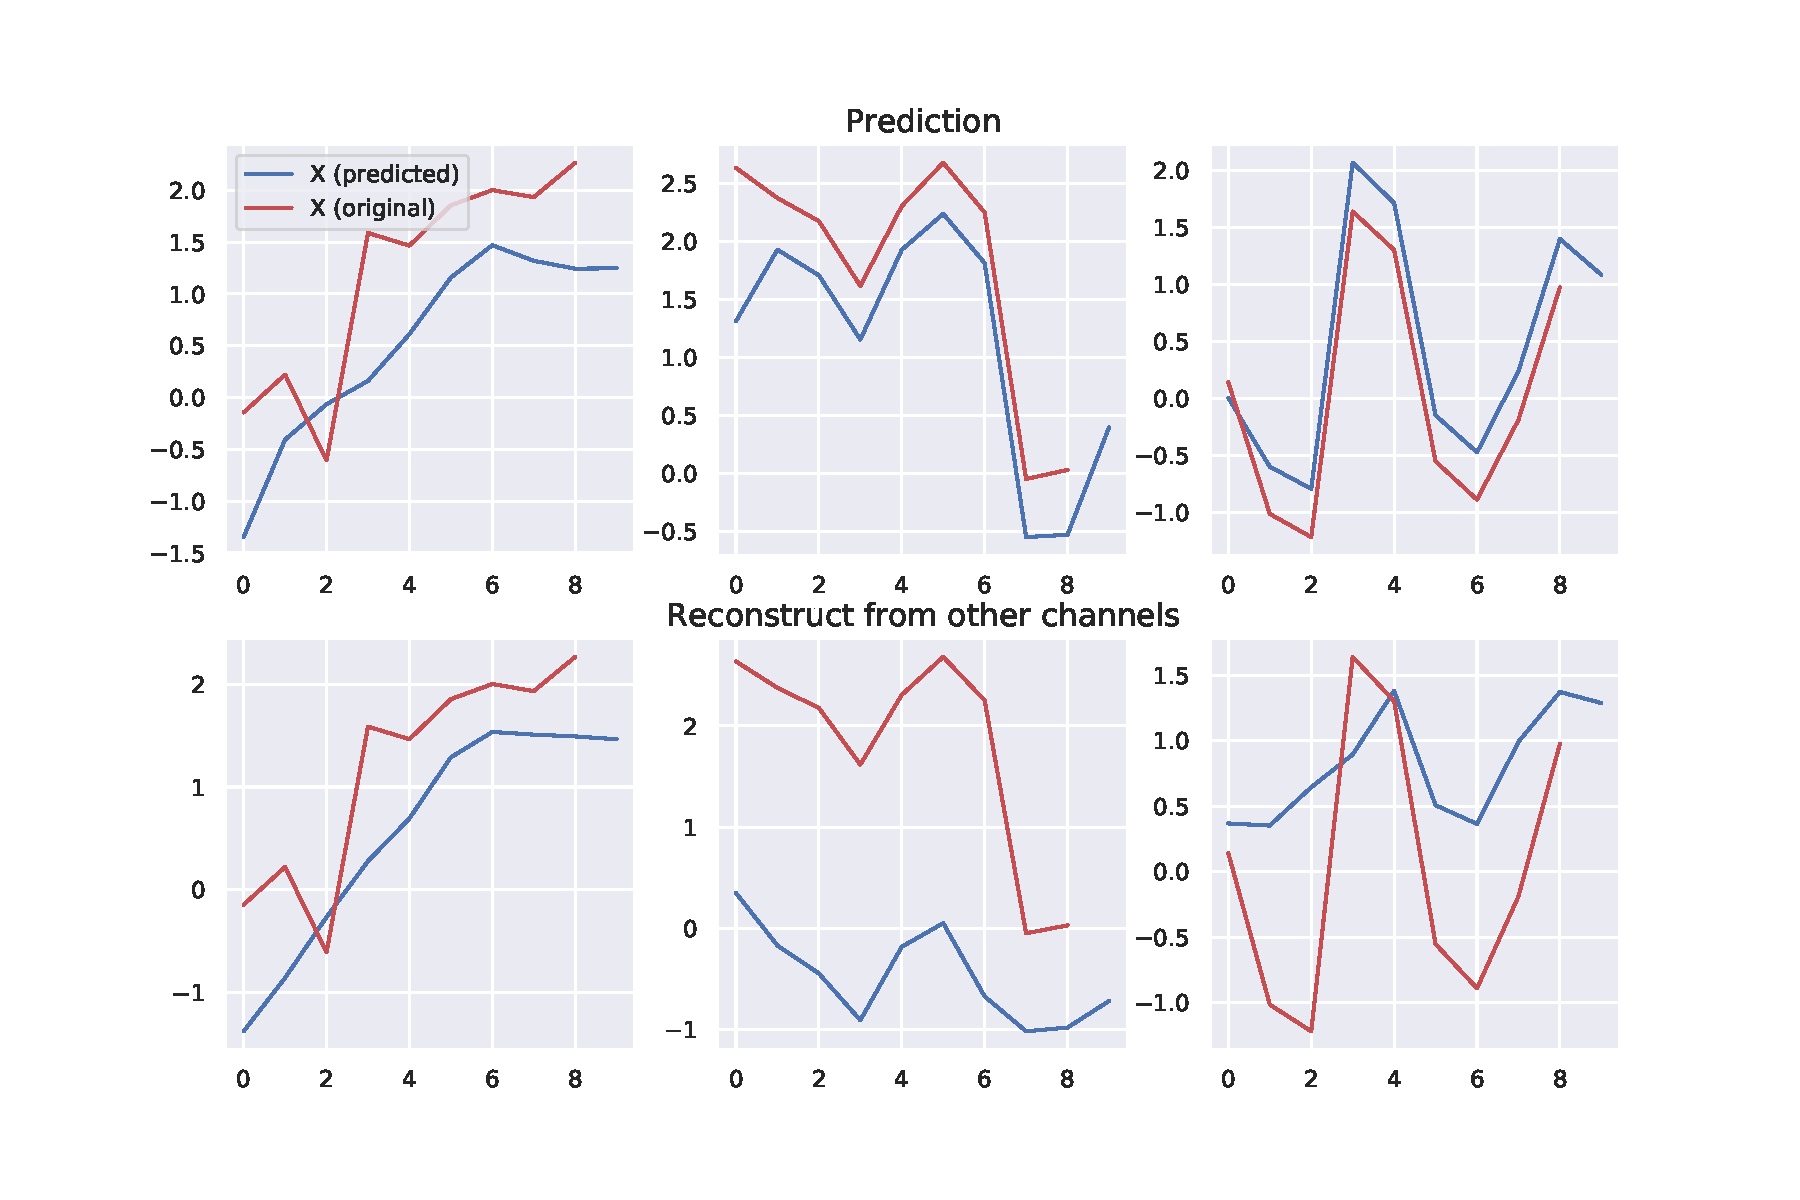
\includegraphics[width=1.0\textwidth]{figures/rnnvae/synth_recon.pdf}
  \caption[Synthetic data reconstruction.]{Reconstruction of the three channels of the generated synthetic data. Top row: reconstruction using all the channels. Bottom row: reconstruction using the other two channels.}\label{fig:rnn:synth1}
\end{figure}

\begin{figure}[!htbp]
  \centering
  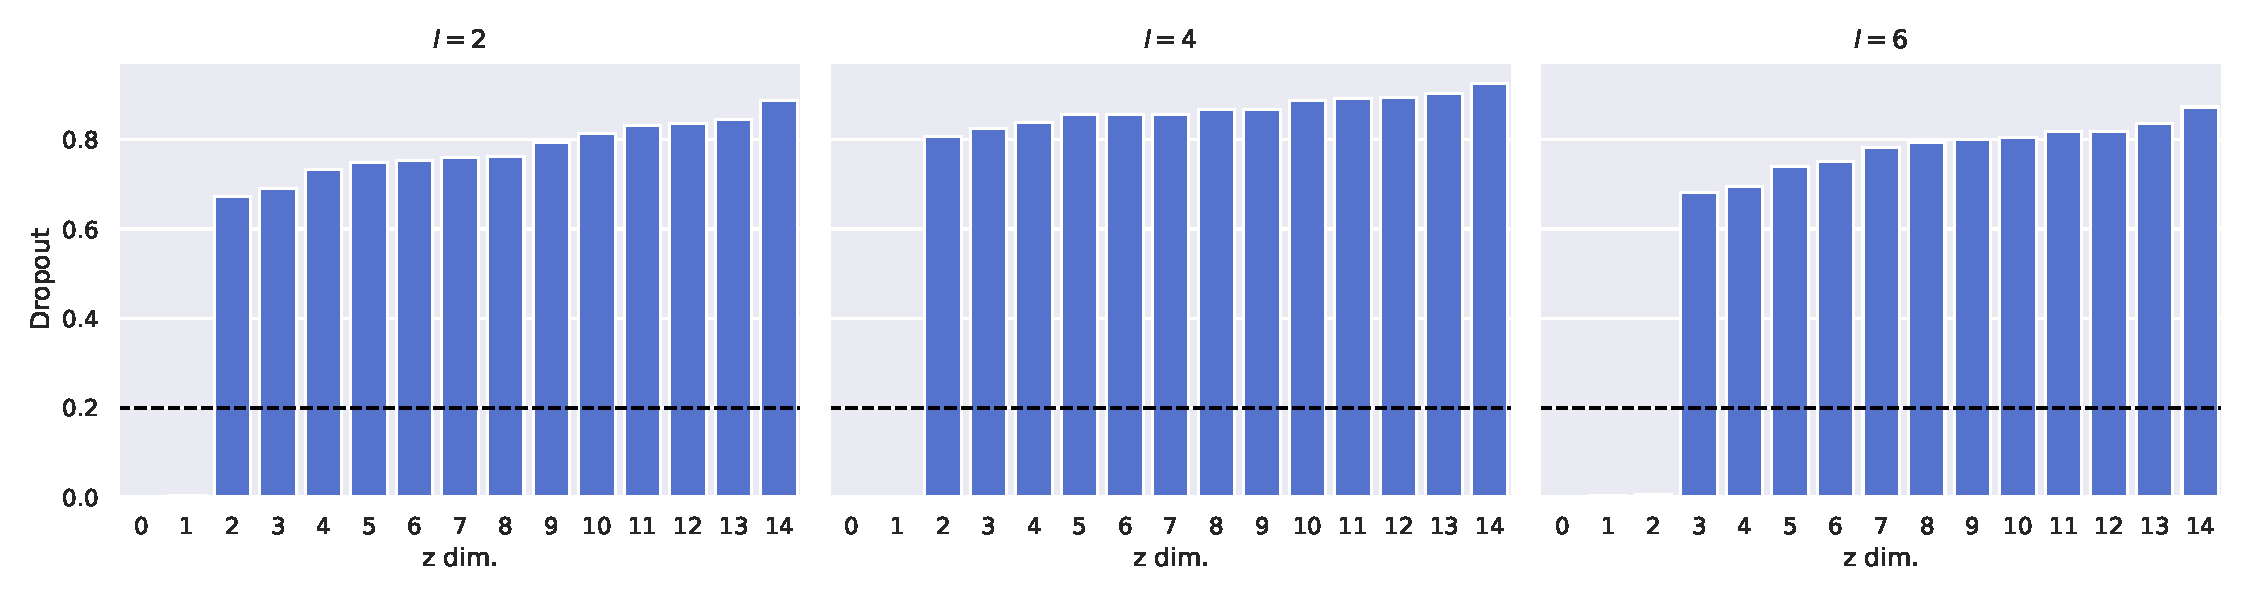
\includegraphics[width=1.0\textwidth]{figures/rnnvae/synthvardrop.pdf}
  \caption[Variational dropout for synthetic data.]{Variational dropout for each latent space dimension of the model, for three different real latent spaces.}\label{fig:rnn:synthvar}
\end{figure}

Regarding the application of variational dropout, Figure \ref{fig:rnn:synthvar} shows the dropout after generating data with different true latent dimensions, compared to the actual latent dimensions of the data. We trained for 3000 epochs with a higher learning rate ($1e-2$)

\subsection{ADNI results}

After hyperparameter optimization, we selected layer size=300, No. latent dim.=20, No. layers=1 and RNN hidden size=300 as the best parameters. Table \ref{table:results:data} shows the results of the two tasks described on the hold-out test set, and compares it to the baseline models described above. We show the results for single-channel and multi-channel models. Figure \ref{fig:rnn:latent} shows the latent space on the test set colored by diagnosis, age, and time point. \\

\begin{table}[!htbp]
\centering
\resizebox{0.95\textwidth}{!}{%
\begin{tabular}{@{}ccccccccc@{}}
\toprule
             & \multicolumn{3}{c}{Long. prediction} & \multicolumn{5}{c}{Channel rec.}      \\ \midrule
             & MRI (vol.)   & MRI (cort.)   & Cog.  & MRI (vol.) & MRI (cort.) & Cog. & Demog. & APOE \\ \midrule
Linear       &  0.240  &  0.395   &  0.486     & -          & -           & -    & -      & -    \\
K-means          & -       & -  & -     &  0.789   &    0.77  & 0.703     & 1.005       &     0.901 \\
RVAE      &  \textbf{0.235}  & \textbf{0.359}  &  \textbf{0.451}  &   -  &     -       & -    &   -    &   -  \\
MC-RVAE &     0.352    &  0.489  & 0.496 &  \textbf{0.691}   &  \textbf{0.687}    &  \textbf{0.608}    & \textbf{0.847} & \textbf{0.885} \\ \bottomrule
\end{tabular}}
\caption[Performance of the model.]{Performance of the models on longitudinal prediction and channel reconstruction, compared to baseline methods. RVAE: single-channel model.  MC-RVAE: multiple channel model. All values are mean absolute error (MAE) over each subject and time point.} \label{table:results:data}
\end{table}


\begin{figure}[!htbp]
  \centering
  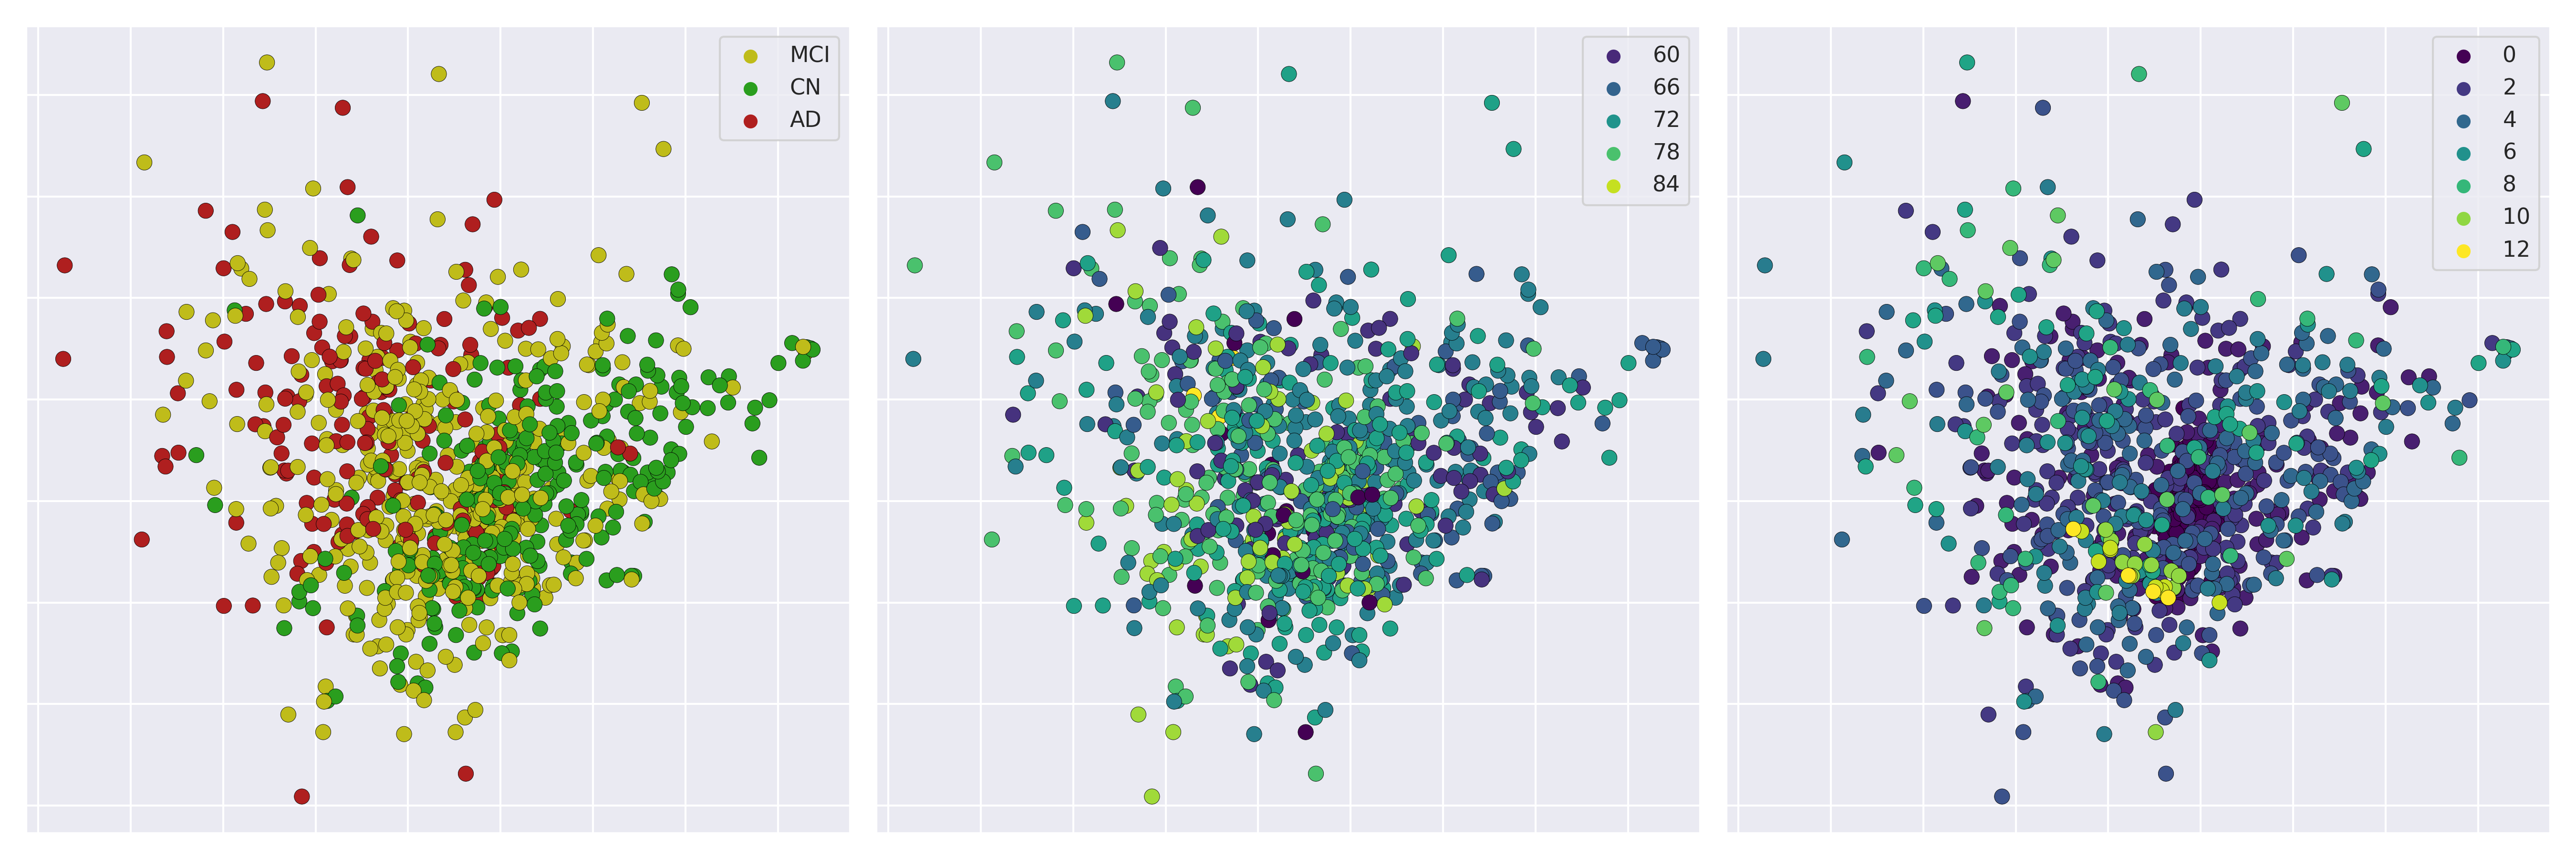
\includegraphics[width=1.0\textwidth]{figures/rnnvae/latent_space_fig.png}
  \caption[Latent space for the test set.]{Dimensions 0 and 1 of the latent space, for subjects on the hold-out test set. Each point represents a different acquisition. Left graphic: colored by diagnosis. Middle: colored by age. Right: colored by time point.}\label{fig:rnn:latent}
\end{figure}

Figure \ref{fig:rnn:qualitative} shows four synthetic time points of cortical and subcortical data. We sampled them using two sequences of 4 cognitive acquisitions: a typical sequence of healthy control and a sequence of a rapidly declining patient, with similar demographic information. Figures were generated using Brainpainter \cite{Marinescu2019a}. The color scale displayed on the figure was obtained by computing the negative z-score of the generated data with respect to a control group of cognitively healthy, amyloid-negative \cite{Shaw2009} patients. \\

\begin{figure}[!htbp]
  \centering
  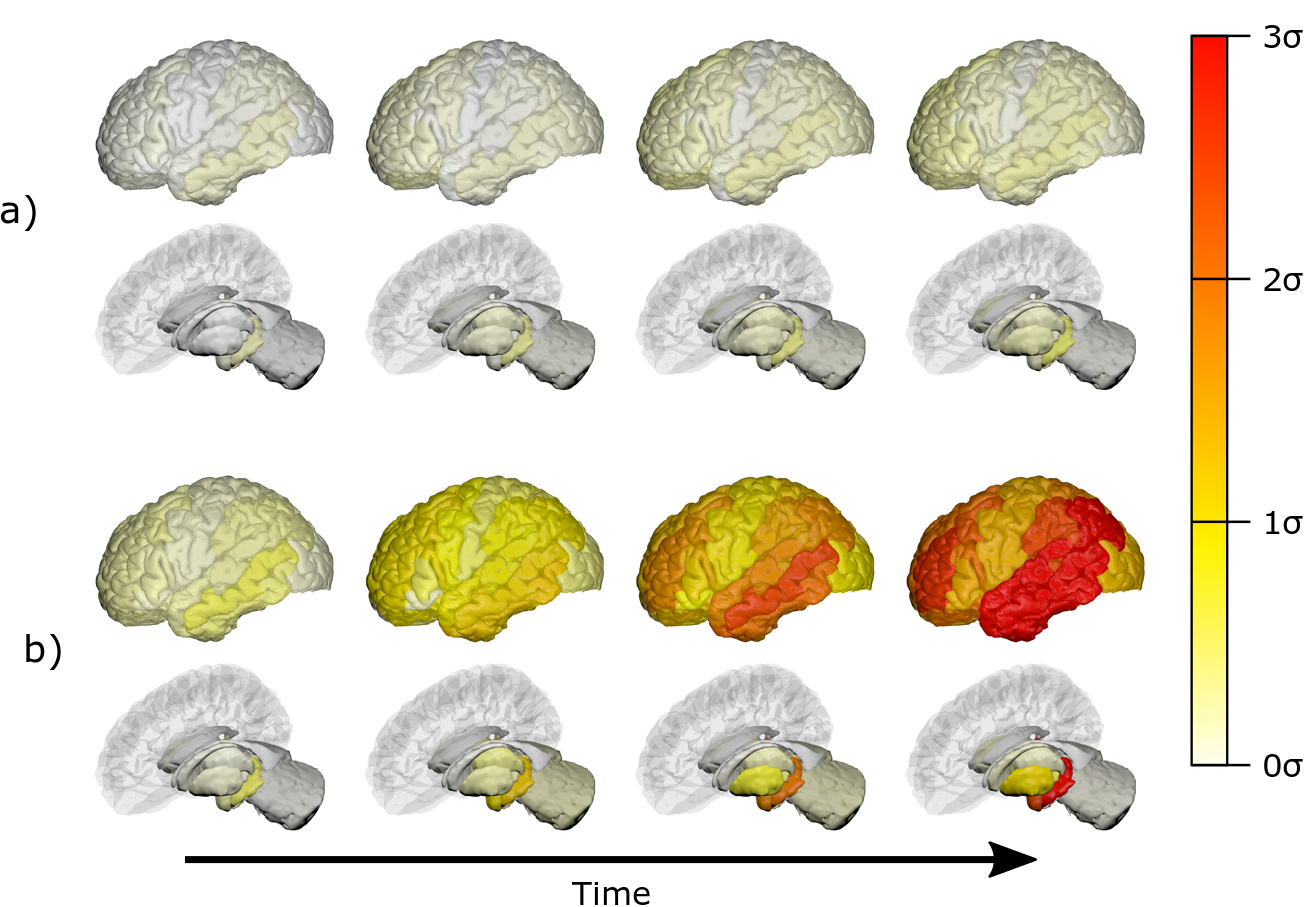
\includegraphics[width=1.0\textwidth]{figures/rnnvae/brainpainter.png}
  \caption[Trajectories of synthetic cortical and subcortical generated by RNN-MCVAE.]{Trajectories of synthetic cortical and subcortical generated by RNN-MCVAE. $\sigma$: standard deviation with respect to the control population. a) and b) corresponds to the two patients described in the main text.}
 \label{fig:rnn:qualitative}
\end{figure}

\section{Discussion}
\label{rnn:discussion}

% Introducció curta del paper.
In this chapter, we proposed a generative method based on recurrent variational autoencoders that is able to jointly model a latent trajectory from multimodal, longitudinal data. We introduced the main concepts and assumptions behind the model, derived its lower bound, and tested it both on synthetic and real data from a cohort of patients afflicted by AD. \\

In our synthetic tests, we show the strength of the method for reconstructing longitudinal signals (Figure \ref{fig:rnn:synth1}). Even in the cases where no information about the original channel is fed to the model, it is still able to reconstruct the general trajectory and direction changes of the signal by using information from other channels (Figure \ref{fig:rnn:synth1}, bottom row). However, the effect of variational dropout in our model is still not clear, as we show in Figure \ref{fig:rnn:synthvar}. The number of latent dimensions selected does not vary alongside the real latent dimensions. Variational dropout in our model needs to be further addressed and adapted to the temporal structure of the latent space, and we have decided not to use it in the tests using the ADNI cohort until more testing is carried out.  \\

For the ADNI cohort, we compared the performance of our model on reconstructing each channel from the others, and on predicting the next time point. Table \ref{table:results:data} shows the results when using a single-channel model for each modality, and using the joint model. For channel reconstruction, the MC-RVAE outperforms the single-channel model, but for prediction, the latter is better. This lower performance could be caused by the increased complexity of all dependencies. Performance could likely be improved by further hyperparameter and model exploration. The latent space generated in the joint model, shown in Figure \ref{fig:rnn:latent}, shows a good separation between diagnosis and age, but we do not appreciate a distinct temporal structure.  \\

To demonstrate the reconstruction capability of the model, Figure \ref{fig:rnn:qualitative} shows two different sequences of cortical and subcortical MRI data generated by the network, for a cognitive healthy patient and a rapidly declining patient. The generated data present a plausible decline of cortical thickness and subcortical volume for both cases, remaining consistent alongside the individual trajectory of the subject. Subject a) shows stability across time for a stable cognitive trajectory, while subject b) shows a rapid decline on the hippocampus and across the cortex, specially in the temporal cortex, which are areas known to be directly affected by AD \cite{Bakkour2013}. \\

% Comparació amb d'altres papers? com enfoquen les discussions?
Compared to existing methods, our model principal contribution is its flexibility to scale to a larger number of channels and a variable number of time points. Cao et al.\ \cite{Cao2019} model, which is based on canonical correlation analysis, can only use two different longitudinal channels, and it is not a generative model. Compared to the multi-channel model of Antelmi et al.\ \cite{Antelmi2019}, from which our model is build upon, our implementation includes temporal structure and allows for temporal data to be included and generated. \\

\section{Conclusions}
\label{rnn:conclusions}

We developed and tested a generative model on multimodal, longitudinal data based on recurrent variational autoencoders. The model is able to combine different modalities of variable length longitudinal data, predict future data, and reconstruct missing modalities. Current results show that the model has potential for missing data reconstruction and prediction tasks. The model performance and architecture, however, requires further development and testing, which is currently underway. Implementing variational dropout adapted to the temporal structure to the latent space would regularize the method and sparsify the latent space, improving both interpretability and performance. We should also test the robustness of our model to predict more than one time point, or how the changes of performance with larger rates of missing data at each time point. Another hindrance of our model is the assumption of equal time between acquisitions. Concrete temporal information could allow the model to sample synthetic data at specific future points, which could be of use for clinical trial design. Finally, we should take advantage of the uncertainty learnt by the model to understand for which tasks and situations the model has less confidence, and improve on it.  \\